\documentclass[tikz,border=10pt]{standalone}
% Scale: s = 0.008511 cm/px, origin at C, y flipped
\begin{document}
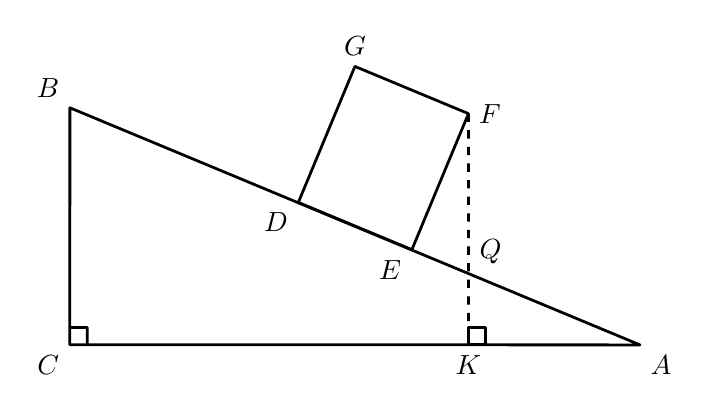
\begin{tikzpicture}[line join=round, line width=1.0pt,
  lbl/.style={font=\fontsize{10}{12}\selectfont}]

% Named points (converted from image px)
\coordinate (C) at (-0.0001023908876240931,0.0007383669865455023);
\coordinate (A) at (7.240022157680597,-0.0005333495211421457);
\coordinate (B) at (0.00042631773914747484,3.010777384792658);
\coordinate (K) at (5.061813982789223,-0.00015075067569303435);
\coordinate (D) at (2.9016045723591186,1.808369209978676);
\coordinate (E) at (4.343686702782224,1.2085349795721987);
\coordinate (F) at (5.062329756881231,2.9362494945750957);
\coordinate (G) at (3.620247626458125,3.536083724981572);
\coordinate (Q) at (5.069971274197959,0.8999309393100887);

% Triangle
\draw (B) -- (C) -- (A) -- cycle;

% Rectangle DGFE (solid)
\draw (D) -- (G) -- (F) -- (E) -- cycle;

% Dashed altitude F to K (through Q)
\draw[dashed] (F) -- (K);

% Right-angle marks (one each)
% Mark at C (unchanged)
\draw (0.21989760571861522,0.0006997243326106734) -- (0.21993624837255005,0.22069972093884996) -- (-0.0000637482336892574,0.2207383635927848);
% Mark at K: closed square (up and right of K, 0.22 units = 26 px)
\draw (K) ++(0,0) -- ++(0,0.22) -- ++(0.22,0) -- ++(0,-0.22) -- cycle;

% Labels
\node[lbl, above left] at (B) {$B$};
\node[lbl, below left] at (C) {$C$};
\node[lbl, below right] at (A) {$A$};
\node[lbl, below] at (K) {$K$};
\node[lbl, above] at (G) {$G$};
\node[lbl, right] at (F) {$F$};
\node[lbl, below left] at (D) {$D$};
\node[lbl, below left] at (E) {$E$};
\node[lbl, above right] at (Q) {$Q$};

\end{tikzpicture}
\end{document}